\setchapterstyle{kao}
\setchapterpreamble[u]{\margintoc}

\chapter{Search for an Excess of Heavy Neutral Lepton Events}
\labch{analysis}

The measurement performed in this thesis is the search for an excess of HNL events in the \SI{10}{years} of IceCube DeepCore data. In principle the two physics parameters to be probed are the mass of the HNL, $m_4$, and the mixing between the fourth heavy mass state and the SM $\tau$ sector, $|U_{\tau4}|^2$. Since the mass itself influences the production and decay kinematics of the event and the accessible decay modes, individual mass sets were produced as described in \refsec{model_specific_simulation}. The mass slightly influences the energy distribution, while the mixing both changes the overall scale of the HNL events and the shape in energy and PID. IceCube DeepCore is suited to measure the excess which appears around and below \SI{20}{\gev}, due to its production from the atmospheric tau neutrinos, although a reduced lower energy threshold could improve the analysis. The measurement will be performed for the three mass sets individually, while the mixing is the parameter that can be varied continuously and will be measured in the fit. 


\section{Final Level Sample} \labsec{analysis_samples}

The final level sample of this analysis always consists of the neutrino and muon MC introduced in \refsec{sm_event_generation} and one of the three HNL samples explained in \refsec{model_specific_simulation}. All of those simulation sets and the \SI{10}{years} of IceCube DeepCore data are processed through the full processing and event selection chain described in \refsec{processing_chain, reconstruction} leading to the final level sample. Since applying the last cuts from \refsec{analysis_cuts} leaves an insignificant amount of pure noise events in the sample, the noise simulation is not included in the analysis and won't be listed here.


\todo{add information about the matter profile used }
\todo{add information about the oscillation probability calculation and the software used for it}

\subsection{Expected Rates/Events}

The rates and the expected events in \SI{10}{years} are shown in \reftab{combined_final_level_expectation}. For the HNL the expectation depends on the mass and the mixing. Shown here are two example mixings for all the three masses. A mixing of $0.0$ would result in a rate of $0.0$ and therefore no HNL events.

\begin{table}
    \begin{tabular}{ llcc }
    \hline\hline

    \textbf{Type} & \textbf{Rate [\si{\milli\hertz}]} & \multicolumn{2}{c}{\textbf{Events (in \SI{10}{years})}} \\ 

    \hline\hline

    $\nu_\mu^\rm{CC}$   & 0.3522 & \multicolumn{2}{c}{103063 ± 113} \\
    $\nu_e^\rm{CC}$     & 0.1411 & \multicolumn{2}{c}{41299 ± 69} \\
    $\nu_\tau^\rm{CC}$  & 0.0348 & \multicolumn{2}{c}{10187 ± 22} \\
    $\nu_\rm{NC}$       & 0.0667 & \multicolumn{2}{c}{968 ± 57} \\
    $\mu$               & 0.0033 & \multicolumn{2}{c}{19522 ± 47} \\
    \hline
    HNL & & \textbf{$|U_{\tau4}|^2=10^{-3}$} & \textbf{$|U_{\tau4}|^2=10^{-1}$} \\ 
    \hline
    $m_4$=\SI{0.3}{\gev} & x.xxx & 2.5 & 1342.5\\
    $m_4$=\SI{0.6}{\gev} & x.xxx & 9.0 & 1207.0\\
    $m_4$=\SI{1.0}{\gev} & x.xxx & 9.6 & 966.5 \\
    
    \hline
    \end{tabular}
\caption[Final level event/rate expectation]{Final level rates and event expectation of the SM background particle types and the HNL signal for all three masses and two example mixing values.}
\labtab{combined_final_level_expectation}
\end{table}

\todo{get correct final level rates from my pipeline(s)}
\todo{add rate and poisson error for HNL samples}
\todo{maybe just pick one mixing?}

\subsection{Analysis Binning}

The identical binning to the analysis performed in \sidecite{flercnn_analysis_result} is used. It was chosen such that the track-like bin has the largest $\nu_\mu$-CC fraction. Extend the binning towards lower energies or increasing the number of bins did not improve the HNL sensitivities significantly. It also has to be considered that sufficient data events need to end up in the individual bins to result in a good fit, which was already investigated in the previous analysis. To mitigate the low data statistics, a few bins were not taken into account in the analysis. There are three bins in PID (cascade-like, mixed and track-like), 12 bins in reconstructed energy, and 8 bins in cosine of the reconstructed zenith angle as specified in \reftab{analysis_binning}. Originally, there were two more bins in $\cos(\theta)$, which were removed to reduce muons coming from the horizon and some low energy bins in the cascade-like bin are removed due to the low event expectation.

\begin{table}
        \begin{tabular}{ llll }
        \hline\hline
    
        \textbf{Variable} & \textbf{$N_\rm{bins}$} & \textbf{Edges} & \textbf{Step} \\ 
    
        \hline\hline
    
        $P_\nu$ & 3 & [0.00, 0.25, 0.55, 1.00] & linear \\
        $E$ & 12 & [5.00, 100.00] & logarithmic \\
        $\cos(\theta)$ & 8 & [-1.00, 0.04] & linear \\
    
        \hline
        \end{tabular}
    \caption[Analysis binning]{Three dimensional binning used in the analysis. All variables are from the FLERCNN reconstruction explained in \refsec{reconstruction}.}
    \labtab{analysis_binning}
\end{table}


\todo{add 3D expectation and/or S/sqrt(B) plots}


\section{Statistical Analysis} \labsec{analysis_principle}


\subsection{Test Statistic}

The measurements are performed by comparing the weighted MC to the data. Through variation of the nuisance and physics parameters that govern the weights, the best matching set of parameters can be found. The comparison is done using a modified $\chi^2$ defined as
\begin{equation}
    \small
    \chi^2_{\mathrm{mod}} = 
    \sum_{i \in \mathrm{bins}}^{}\frac{(N^{\mathrm{\nu}}_i + N^{\mathrm{\mu}}_i + N^{\mathrm{HNL}}_i - N^{\mathrm{obs}}_i)^2}
    {N^{\mathrm{\nu}}_i + N^{\mathrm{\mu}}_i + N^{\mathrm{HNL}}_i + (\sigma^{\mathrm{\nu}}_i)^2 + (\sigma^{\mathrm{\mu}}_i)^2 + (\sigma^{\mathrm{HNL}}_i)^2}
     + \sum_{j \in \mathrm{syst}}^{}\frac{(s_j - \hat{s_j})^2}{\sigma^2_{s_j}}
    \;,
    \labeq{mod-chi2-hnl}
\end{equation}
as the test statistic (TS), where $N^{\mathrm{\nu}}_i$, $N^{\mathrm{\mu}}_i$, and $N^{\mathrm{HNL}}_i$ are the expected number of events in bin $i$ from neutrinos, atmospheric muons, and HNL, while $N^{\mathrm{obs}}_i$ is the observed number of events in bin $i$. The expected number of events from each particle type is calculated by summing the weights of all events in the bin $N^{\mathrm{type}}_i = \sum_i^\rm{type}\omega_i$, with the statistical uncertainty being $(\sigma^{\mathrm{type}}_i)^2 = \sum_i^\rm{type}\omega_i^2$. The expected Poisson error is calculated using the combined expectation of neutrinos, atmospheric muons, and HNL events. The additional term in \refeq{mod-chi2-hnl} is included to apply a penalty term for prior knowledge of the systematic uncertainties of the parameters where they are known. $s_j$ are the systematic parameters that are varied in the fit, while $\hat{s_j}$ are their nominal values and $\sigma_{s_j}$ are the known uncertainties.

\todo{Do I want/need to include the description of the KDE muon estimation?}

\subsection{Systematic Uncertainties} \labsec{analysis_systematics}


\subsubsection{Treatment of Detector Response Uncertainties via a Likelihood-Free Inference Method} \labsec{ultrasurfaces}

\sidecite{Fischer_2023}


Copy paste from OVS PRD about hypersurfaces (and interpolation of those):

To evaluate the expected impact of detection uncertainties, data sets are produced with different variations of detector response, processed to the final level of selection, and then they are parameterized following a model of the uncertainties to evaluate how the final sample would look like for any reasonable choice of parameters. The parametrizations are done at the analysis bin level, assuming that every effect considered is independent and that they can be approximated by a linear function. Under these assumptions we can compute a reweighting factor in every bin that depends on $N$ parameters, which correspond to the number of systematic effects being considered, plus an offset $c$, as

\begin{equation}
    f(p_1,...,p_N)=c+\sum_{n=1}^N m_n \Delta p_n.
\end{equation}
Here $m_n$ are the reweighting factors obtained from simulation sets with a systematic variation and $\Delta p_n$ is the test value of a specific systematic variation.

The fit of the parameters $m_n$ is done over all systematic MC sets, reducing the uncertainty on the MC prediction in each bin as a side effect since the error on the fitted function is smaller than the statistical error from the nominal MC set. The set of all fitted functions in all histogram bins are called ``hypersurfaces". An example of such a fit from a single bin, projected onto one dimension, is shown in Fig. \ref{fig:hypersurface-example}. %The result of using hypersurfaces accurately predicted the bin content of simulation sets that were left out of the parameterization.

The event counts coming from different flavors and interactions have a different response to varying the same detector parameter. Therefore, the hypersurfaces in each bin are fit separately for three groups of events:
\begin{itemize}
    \item ($\nu_{\mathrm{all}} + \bar{\nu}_{\mathrm{all}}$) NC + ($\nu_e + \bar{\nu}_e$) CC: These events all produce cascade signatures in the detector.
    \item ($\nu_\tau + \bar{\nu}_\tau$) CC: These interactions may differ from the previous group because they have a production threshold of $E_\nu \gtrsim 3.5\,\mathrm{GeV}$ and also produce muons with a branching ratio of 17\%.
    \item ($\nu_\mu + \bar{\nu}_\mu$) CC: These interactions produce track-like signatures.
\end{itemize}

% \begin{figure}[t!]
%     \centering
%     \includegraphics[width=.95\linewidth]{Figures/detector_syst/hypersurface_example_v5.pdf}
%     \caption{Example of a hypersurface function in one bin projected on the DOM efficiency dimension. Each data point corresponds to one systematic set. Translucent datapoints are from sets where one or more systematic parameter \emph{besides} DOM efficiency is off-nominal. Those points are projected along the fitted plane to the nominal point. Several systematic sets have a nominal DOM efficiency of 1.0. The translucent error band corresponds to the standard deviation of the fitted function.}
%     \label{fig:hypersurface-example}
% \end{figure}

The distribution of $\chi^{2}$/d.o.f. from the fits in all analysis bins is used as a diagnostic to ensure that the fitted, linear hypersurfaces provide a good estimate for the expected number of events for the full range of simulated detector configurations. We find that the means of these $\chi^{2}$/d.o.f. distributions are all consistent with 1.0 as expected from good fits for each of the three categories described above (NC + $\nu_{e}$ CC, $\nu_{\tau}$ CC and $\nu_{\mu}$ CC). Attempts to use higher order polynomial fits did not yield a significantly improved $\chi^{2}$/d.o.f., and in fact often rendered the fits less stable. 

To produce the histograms for fitting the hypersurfaces, a choice must be made for the values of flux, cross section and oscillation parameters. We found that the hypersurface fits are sensitive to the choice of parameters that have correlations with the effect they encode. Most notably, this effect is observed between the mass splitting and DOM optical efficiency as demonstrated in Fig.~\ref{fig:interpolatedHS}, which shows the difference between fitted hypersurface gradients for the DOM efficiency dimension for two values of $\Delta m^{2}_{32}$. 
%Moreover, we found that assuming the wrong mass splitting can introduce a significant bias in the measurement if the fitted DOM efficiency is pulled by only 1$\sigma$. 

This problem arises because we are only fitting the hypersurfaces in reconstructed phase space, without accounting for the different true energy and zenith distributions of MC in each analysis bin, which change with each detector systematic variation. To mitigate this problem, we fit the hypersurfaces for 20 different values in mass splitting between $1.5\times 10^{-3}\,\mathrm{eV}^2$ and $3.5\times 10^{-3}\,\mathrm{eV}^2$, and then apply a piece-wise linear interpolation to all slopes, intercepts and covariance matrix elements. The oscillation parameter fit can then dynamically adapt the hypersurfaces for each value of $\Delta m^{2}_{32}$ that is tested using these interpolated functions. The effects of other parameter choices were evaluated as well, but none were found to introduce a significant bias.


\subsubsection{Free Parameter Selection} \labsec{parameter_selection}





Copy paste from OVS PRD about systematic impact test:

We decide which systematic uncertainties must be included in the fit by studying the potential bias they would produce in the oscillation parameters and the change on the test statistic $\chi^2_\mathrm{mod}$ if we neglected them. We create data sets with their observed quantities set equal to their expected values for a wide range of values for $\theta_{23}$ and $\Delta m^{2}_{32}$ and perform two fits: one where the oscillation parameters are fixed to their true value and one where they are left free. In both fits, the systematic parameter being tested is fixed to a value off from its nominal expectation by either 1$\sigma$ or by an educated guess, if the uncertainty is not well-defined. Parameters are included in the analysis when this test creates a significant bias in the oscillation parameters, which is conservatively defined as a difference larger than $2\times10^{-2}$ between the test statistics of the two fits.

Copy paste from OVS PRD about detector systematic nominal, prior, and ranges:

As motivated in Section~\ref{sec:detector_calibration}, the DOM efficiency is constrained by a Gaussian prior to the value of 1.0 $\pm$ 0.1. The ice model parameters are unconstrained in the fit, and allowed to vary within conservative ranges determined from calibration data. The hole ice model parameters are bounded within the ranges $-2.0<p_{0}<1.0$ and $-0.2<p_{1}<0.2$. The bulk ice model parameters are bounded within $-0.90 < \mathrm{Absorption} < 1.10$ and $-0.95 < \mathrm{Scattering} < 1.15$.

\todo{Add table with all systematic uncertainties used in this analysis (in the analysis chapter).}
\todo{add final level effects of varying the axial mass parameters (or example of one)}
\todo{add final level effects of varying the DIS parameter (or example of one)}

\section{Analysis Checks}

Fitting to data will be performed in a \textit{blind} manner, where the analyzer does not immediately see the fitted physics and nuisance parameter values, but first checks that a set of pre-defined \textit{goodness of fit (GOF)} criteria are fulfilled. If those criteria are met to satisfaction the fit results are unblinded and the full result can be revealed. Before these blind fits to data are run, the robustness of the analysis method is tested using pseudo-data that is generated using the MC sets.


\subsection{Asimov Inject/Recover Tests}

- descibe used minimizer and minimization routine
- minimize the modified $\chi^2$ TS
- describe the Asimov data set (no statistical fluctuations)
- without fluctuations the fit is always expected to recover the injected parameters
- \reffig{asimov_inject_recover_0.6_GeV}

\begin{figure}
    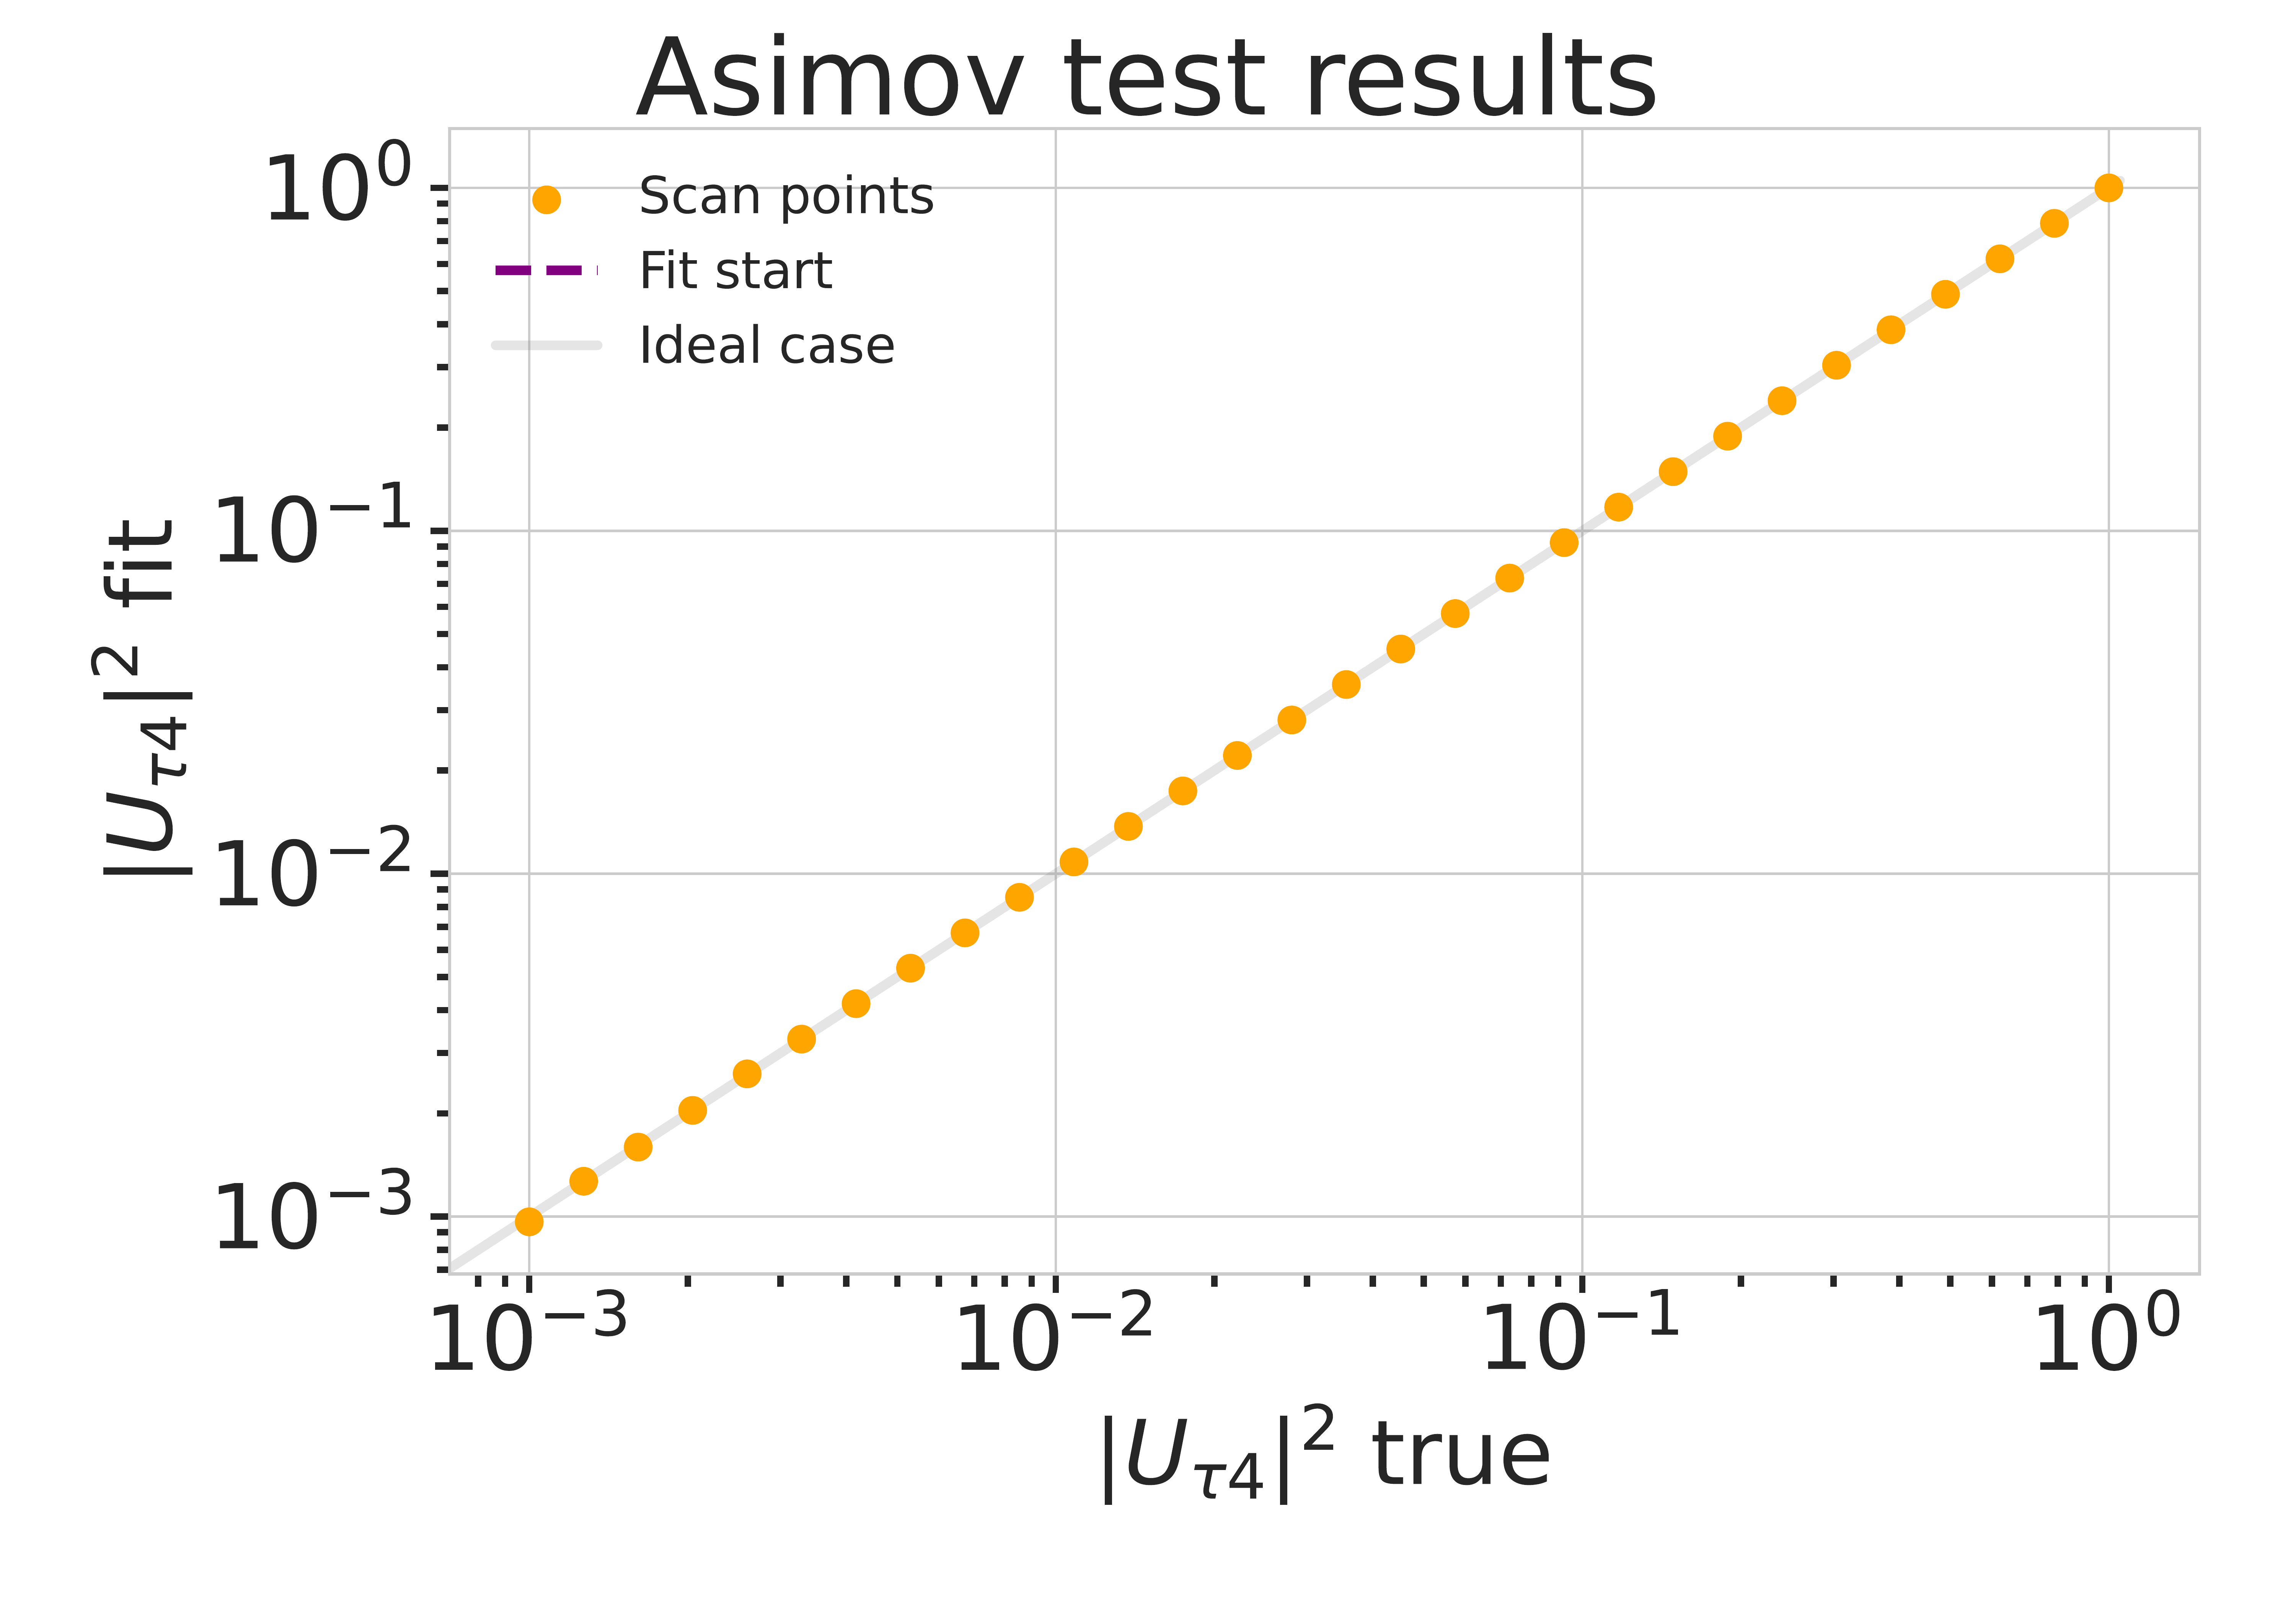
\includegraphics{figures/results/checks/asimov_scan_0.6_GeV-01.png}
	\caption[Asimov inject/recover test (\SI{0.6}{\gev})]{Asimov inject/recover test for the \SI{0.6}{\gev} mass set. Mixing values between $10^{-3}$ and $10^{0}$ are injected and fit back with the full analysis chain. The injected parameter is alwasy recovered within the statistical uncertainty.}
    \labfig{asimov_inject_recover_0.6_GeV}
\end{figure}

\todo{put in asimov inject/recover plots for other masses in the appendix}


\subsection{Sensitivity}

\subsection{Ensemble Tests}


\section{Results}

\subsection{Best Fit Parameters}

\subsection{Upper Limits}

\subsection{Post-Fit Data/MC Agreement}
